\section{Introduction} 
\par Battery electric buses (BEBs) are replacing diesel and natural gas buses in public transportation because BEBs offer many benefits \cite{Mahmoud2016} including reduced maintenance \cite{poornesh_comparative_2020}, zero emissions \cite{kato_comparative_2013}, and access to renewable energy \cite{cheng_smart_2020}.  The challenge of prolonged charging times has been addressed in prior research including distributed charging networks \cite{Nimalsiri2020}, bus availability, environmental impact \cite{zhou_bi-objective_2021}, route scheduling \cite{Rinalde_Mixed_2020}, battery health \cite{houbbadi_optimal_2019}, the cost of electricity \cite{Leou_optimal_2017}, and the cost of charging infrastructure \cite{Wei2018}.  
\par Because charge times can be lengthy, some prefer to use high power chargers, which deliver more energy in a smaller period of time. However doing so places large power demands on electrical infrastructure \cite{stahleder_impact_2019} so that power networks become unreliable \cite{deb_impact_2017} and expensive because high power requires additional maintenance and upgrades \cite{boonraksa_impact_2019}. An effective charge plan must therefore balance the need to charge quickly with the desire to maintain a low power profile \cite{ojer_development_2020}.  
\par Methods for developing charge plans range from heuristic approaches \cite{qin_numerical_2016}, to network flow on a graph \cite{whitaker_network_2023}, to reinforcement learning\cite{Wang2019}, to mixed integer linear programs (MILP) \cite{bagherinezhad_spatio-temporal_2020}. Generally, each method minimizes cost by either decreasing the instantaneous power needs for the fleet, or optimizing around time-of-use tarrifs \cite{He_2019_Fast}.  
\par Scaling these methods to large bus fleets ($>$100 BEBs) and numerous chargers is a challenge due to the size of the optimization problem that must be solved.  For small fleets ($<$50 BEBs) and less than 10 chargers, the optimization problems in \cite{whitaker_network_2023,bagherinezhad_spatio-temporal_2020,He_2019_Fast} have over $10^5$ variables (including binary and integer variables) and over $10^5$ constraints.  Scaling to larger fleets and more chargers stresses computational resources and requires lengthy solve times.  
\par This paper continues the main theme of prior work which is to develop charging schedules for electric buses that minimize the monthly electricity bill (energy consumption plus power demand) while satisfying route constraints that demand buses be in specific locations at specific times.  One novelty is that our formulation considers the agregated effects of loading across multiple meters.  While meter agregation is not widespread today, distribution networks must be built to supply worst case loads to each metered circuit.  Therefore, our approach begins to explore how optimization of loads across multilple meters can reduce the overall impact of BEB charging on the grid.  In this work, meter agregation is modeled through the inclusion of uncontrolled (i.e. non-BEB charging) loads.  Specifically, we incorporate historical load data from an electric train (UTA TRAX) that visits a central intermodal hub transit site in Salt Lake City, Utah which is also a charging stop for BEBs.  
\par The main contribution of the present paper is addressing the matter of scale.  Rather than posing a single large MILP that incorporates every aspect of the charging problem, we solve a series of small subproblems in which the solution to the charging problem becomes successively more refined and moves closer to the optimal schedule.  Our results show that the intermediate subproblems can be solved with a dramatic reduction in runtimes allowing our method to be applied to significantly larger bus fleets.  In a sense, this work explores what is gained in runtime by sacrificing some optimality in the schedule.  The subproblems fall into three groups as shown in Fig. \ref{fig:processChain}.  Each sub-problem is solved using a linear, quadratic, or integer program and when used together the series of programs provides a near optimal charge plan. Each sub-problem addresses elements from one of three areas: energy allocation and bus grouping, session length and bus-to-charger assignments, and second-by-second optimization.  

\subsection{Energy Allocation and Group Assignment} 
\par The first set of problems answers two primary questions: (1) at what time should energy be delivered to each bus, and (2) which buses are most able to share chargers.  These questions are addressed through three sub-problems: unconstrained charge schedule, smooth charge schedule, and group separation.  
\par The unconstrained schedule problem (denoted $P_1$) is described in Section \ref{sec:unconstrainedSchedule} computes an optimal charge schedule which minimises the monthly cost of power in the presence of uncontrolled loads under the assumption that each bus has a dedicated charger.  
\par The smooth schedule problem (denoted $P_2$) is described in Section \ref{sec:unconstrainedSmoothSchedule} has the same form as $P_1$ with two differences.  First, the monthly cost is required to match the optimal cost from the solution to the unconstrained scheduling problem. Second, the objective for the smooth schedule problem penalizes change in the scheduled charge rates. {\textbf Use the problem names $P_x$ here.}
\par The group assignment problem (denoted $P_3$) is described in Section \ref{sec:groupAssignment} uses the charge schedules from $P_2$ to separate buses into groups such that the bus schedules within a group overlap as little as possible.  Separating the scheduling problem into groups helps to manage the number of computations in succeeding optimization problems by reducing the size of these problems.

\subsection{Session Time and Charger Assignment} 
The problems in the session time and charger assignment section are computed on a per-group basis to reduce the number of computations, address two questions: (1) when should charge sessions start and stop, and (2) which charger should be used for each session.  These questions are answered through three sub-problems: defragmentation, charger assignment, and session refinement.

\par The defragmentation problem (denoted $P_4$) is described in Section \ref{sec:defragmentation} attempts to consolidate charge sessions with small amounts of energy to reduce the number of charge sessions and serves to both decrease the computational complexity of the charger assignment problem by reducing the number of charge sessions and simplify the charge schedule to make it more operationally feasible.  
\par After consolidation, each charge session is defined by a minimum/maximum start/stop time as given by the bus's arrival and departure times and an energy requirement in kW. The charger assignment problem (denoted $P_5$) is described in Section \ref{sec:chargerAssignment} uses the availability and energy constraints to assign chargers to charge sessions.  
\par Once charge sessions are placed, the final step is to ensure each session makes the most of each charger's availability. Many times, especially when using non-optimal gaps in the charger assignment problem, the charge schedules may not use all available time on a charger. The charger refinement problem (denoted $P_6$) expands each charge session to fill unused time on either side and prioritizes sessions with higher energy demands for adjacent sessions.  

\subsection{Final Optimization} 
Solutions to the previous problems provide a set of charge sessions, energy requirements, and time schedules for specific chargers. The final question to be answered is how should the energy for each session will be delivered. The two sub-problems in the final optimization section mirror problems $P_1$ and $P_2$ from the energy allocation and group assignment sections. The first problem (denoted $P_7$), uses the energy and time constraints from previos solutions to compute an optimal charge schedule in Section \ref{sec:constrainedSchedule} and is analagous to the unconstrained charge problem $P_1$. The second problem (denoted $P_8$) computes a smoothed charge schedule with the same cost as the constrained schedule solution in Section \ref{sec:constrainedSmoothSchedule} and is analagous to the smooth charge schedule problem $P_2$ in Section \ref{sec:unconstrainedSmoothSchedule}. The table given in Fig.~\ref{fig:formulation:features} lists each problem and which features each problem incorporates.

\begin{figure*}\centering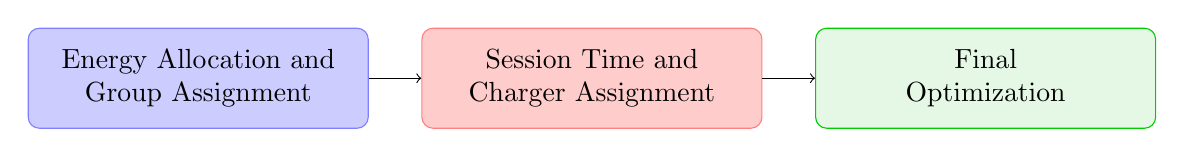
\begin{tikzpicture}
	\node[rectangle, draw=blue!50, fill=blue!20, minimum width=1.7in, minimum height=0.5in, rounded corners](set1) at (0,0) {\begin{tabular}{c} Energy Allocation and\\ Group Assignment\end{tabular}}; 
	\node[rectangle, draw=red!50, fill=red!20, minimum width=1.7in, minimum height=0.5in, rounded corners](set2) at (5,0) {\begin{tabular}{c} Session Time and \\Charger Assignment \end{tabular}}; 
	\node[rectangle, draw=green!80!black, fill=green!70!black!10, minimum width=1.7in, minimum height=0.5in, rounded corners](set3) at (10,0) {\begin{tabular}{c} Final \\ Optimization\end{tabular}}; 
	\draw[->] (set1.east) -- (set2.west);
	\draw[->] (set2.east) -- (set3.west);
\end{tikzpicture}\caption{Overall Processing Chain}\label{fig:processChain}\end{figure*}

 
\begin{figure*}\centering\scalebox{0.8}{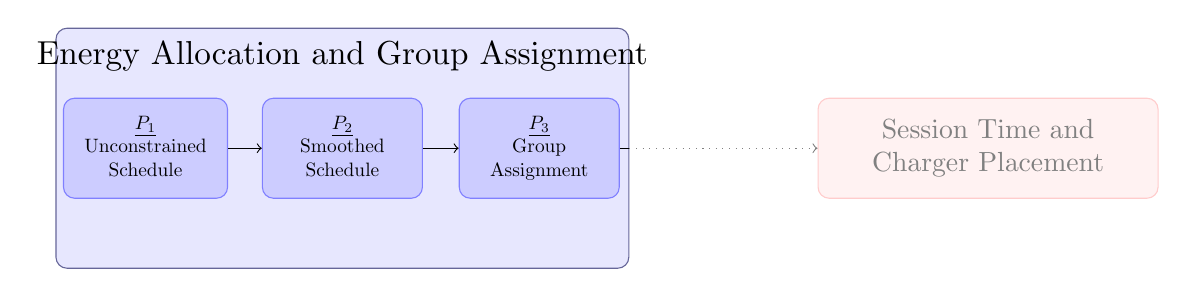
\begin{tikzpicture}
\node[rectangle, draw=gray!80!blue, fill=gray!10!blue!10, minimum width=\textwidth*0.6, minimum height=1.2in, rounded corners, label={[label distance=-0.67cm]above:\scalebox{1.2}{Energy Allocation and Group Assignment}}](outline) at (0,0){};
	\node[rectangle, draw=blue!50, fill=blue!20, minimum width=0.8in, minimum height=0.5in, rounded corners](problem1) at (-2.5,0) {\scalebox{0.7}{\begin{tabular}{c} \underline{$P_1$} \\ Unconstrained \\ Schedule\end{tabular}}}; 
	\node[rectangle, draw=blue!50, fill=blue!20, minimum width=0.8in, minimum height=0.5in, rounded corners](problem2) at (0,0) {\scalebox{0.7}{\begin{tabular}{c}\underline{$P_2$} \\  Smoothed \\ Schedule\end{tabular}}}; 
	\node[rectangle, draw=blue!50, fill=blue!20, minimum width=0.8in, minimum height=0.5in, rounded corners](problem3) at (2.5,0) {\scalebox{0.7}{\begin{tabular}{c}\underline{$P_3$} \\ Group \\ Assignment\end{tabular}}}; 
	\node[rectangle, draw=red!20, fill=red!5, text=black!50, minimum width=1.7in, minimum height=0.5in, rounded corners](problem4) at (8.2,0){\begin{tabular}{c}Session Time and \\ Charger Placement\end{tabular}};
	\draw (problem3.east) -- (outline.east);
	\draw[->, draw=black!50, dotted] (outline.east) -- (problem4.west);
	\draw[->, draw=black] (problem1.east) -- (problem2.west);
	\draw[->, draw=black] (problem2.east) -- (problem3.west);
\end{tikzpicture}}\caption{Processing chain for the energy allocation and group assignment problems} \label{fig:set1Chain}\end{figure*}

 
\begin{figure*}\centering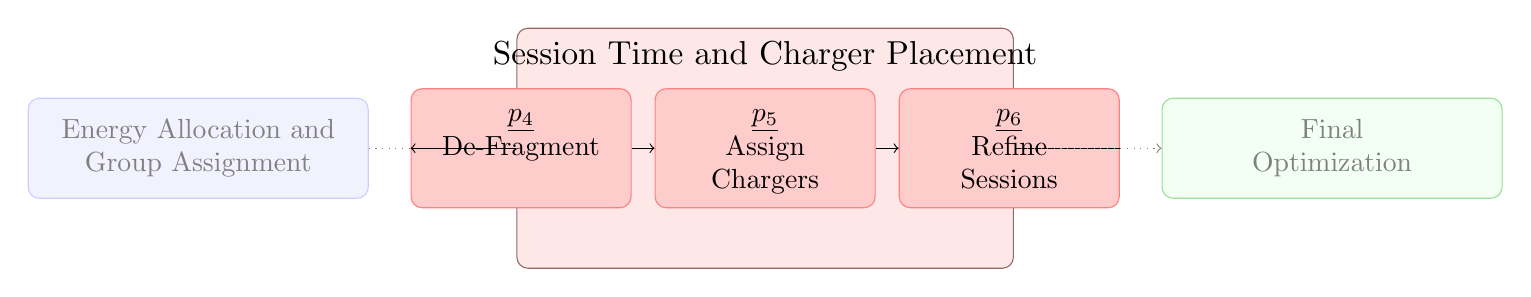
\begin{tikzpicture}
\node[rectangle, draw=gray!80!red, fill=gray!10!red!10, minimum width=\textwidth*0.52, minimum height=1.2in, rounded corners, label={[label distance=-0.67cm]above:\scalebox{1.2}{Session Time and Charger Placement}}](outline) at (0,0){};
	\node[rectangle, draw=red!50, fill=red!20, minimum width=1.1in, minimum height=0.5in, rounded corners](problem1) at (-3.1,0) {\begin{tabular}{c} \underline{$p_4$} \\ De-Fragment \\  \\\end{tabular}}; 
	\node[rectangle, draw=red!50, fill=red!20, minimum width=1.1in, minimum height=0.5in, rounded corners](problem2) at (0,0) {\begin{tabular}{c}\underline{$p_5$} \\ Assign\\ Chargers\end{tabular}}; 
	\node[rectangle, draw=red!50, fill=red!20, minimum width=1.1in, minimum height=0.5in, rounded corners](problem3) at (3.1,0) {\begin{tabular}{c}\underline{$p_6$} \\ Refine\\ Sessions\end{tabular}}; 
	\node[rectangle, draw=blue!20, fill=blue!5, text=black!50, minimum width=1.7in, minimum height=0.5in, rounded corners](problem0) at (-7.2,0){\begin{tabular}{c}Energy Allocation and\\ Group Assignment\end{tabular}};
	\node[rectangle, draw=green!70!black!40, fill=green!5, text=black!50, minimum width=1.7in, minimum height=0.5in, rounded corners](problem4) at (7.2,0){\begin{tabular}{c}Final \\ Optimization\end{tabular}};
	\draw[draw=black!50, dotted] (problem0.east) -- (outline.west);
	\draw[->] (outline.west) -- (problem1.west);
	\draw (problem3.east) -- (outline.east);
	\draw[->, draw=black!50, dotted] (outline.east) -- (problem4.west);
	\draw[->, draw=black] (problem1.east) -- (problem2.west);
	\draw[->, draw=black] (problem2.east) -- (problem3.west);
\end{tikzpicture}\caption{Processing chain for each group} \label{fig:set2Chain}\end{figure*}

 
\begin{figure*}\centering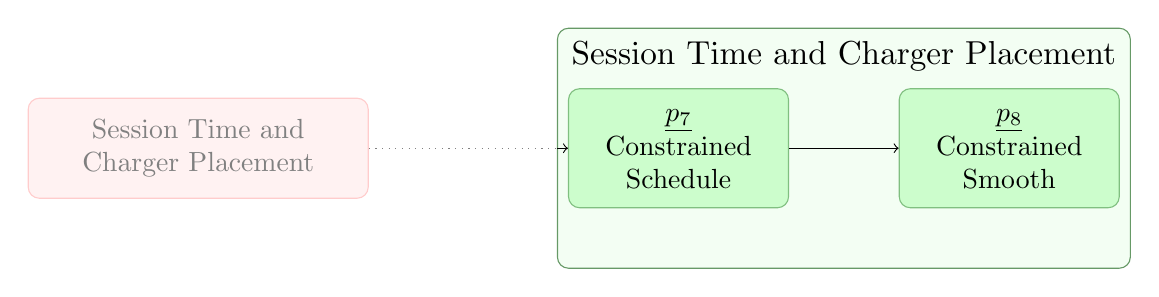
\begin{tikzpicture}
\node[rectangle, draw=gray!80!green, fill=gray!10!green!5, minimum width=\textwidth*0.6, minimum height=1.2in, rounded corners, label={[label distance=-0.67cm]above:\scalebox{1.2}{Session Time and Charger Placement}}](outline) at (0,0){};
	\node[rectangle, draw=green!50!black!50, fill=black!3!green!20, minimum width=1.1in, minimum height=0.5in, rounded corners](problem1) at (-2.1,0) {\begin{tabular}{c} \underline{$p_7$} \\ Constrained \\ Schedule\end{tabular}}; 
	\node[rectangle, draw=green!50!black!50, fill=black!3!green!20, minimum width=1.1in, minimum height=0.5in, rounded corners](problem3) at (2.1,0) {\begin{tabular}{c}\underline{$p_8$} \\ Constrained \\ Smooth\end{tabular}}; 
	\node[rectangle, draw=red!20, fill=red!5, text=black!50, minimum width=1.7in, minimum height=0.5in, rounded corners](problem0) at (-8.2,0){\begin{tabular}{c}Session Time and \\ Charger Placement\end{tabular}};
	\draw[draw=black!50, dotted] (problem0.east) -- (outline.west);
	\draw[->] (outline.west) -- (problem1.west);
	\draw[->, draw=black] (problem1.east) -- (problem3.west);
\end{tikzpicture}\caption{Processing chain for the Final Optimization set} \label{fig:set3Chain}\end{figure*}


\begin{figure*}\label{fig:formulation:features}\centering
\newcommand{\grayhline}{\arrayrulecolor{gray!20} \hline \arrayrulecolor{black}}
\begin{tabular}{l c c c c c c c c}
 Feature                        & $P_1$ & $P_2$ & $P_3$ & $P_4$ & $P_5$ & $P_6$ & $P_7$ & $P_8$ \\ \hline 
Battery State of Charge         &   x   &   x   &       &   x   &       &       &   x   &   x   \\ \grayhline      
Minimize Cost                   &   x   &   x   &       &   x   &       &       &   x   &   x   \\ \grayhline           
Charger Capacity                &   x   &   x   &   x   &   x   &   x   &       &   x   &   x   \\ \grayhline      
Energy Placement                &   x   &   x   &       &   x   &       &       &   x   &   x   \\ \grayhline      
Smooth Charge Plan              &       &   x   &       &       &       &       &       &   x   \\ \grayhline      
Computationally Scalable        &       &       &   x   &       &       &       &   x   &   x   \\ \grayhline      
Small Number of Charge Sessions &       &       &       &   x   &       &       &   x   &   x   \\ \grayhline      
Number of Chargers              &       &       &       &       &   x   &       &   x   &   x   \\ \grayhline      
Efficient Charger Use           &       &       &       &       &       &   x   &   x   &   x   \\ \grayhline      
Precise Charge Plan             &       &       &       &       &       &       &   x   &   x   \\ \grayhline      
\end{tabular} 
\caption{Descriptions of in which problems features are addressed}
\label{fig:formulation:features}
\end{figure*}


